\documentclass[small,algo]{dushClass}


\title{Initialisation aux Frameworks : TP}
\subtitle{Hibernate}

\begin{document}

\section{Installation du poste de travail}

\subsection{Les outils}
\begin{description}
\item[Eclipse] : utiliser la version \emph{SpringSource Tools Suite} qui contient déjà tous les plugins nécessaires.
\item[Maven] : outils de gestion de dépendance, de compilation
\item[HSQL DB] : base de données ne nécessitant pas d'installation
\item[Git] : gestionnaire de version
\item[Cygwin] : console type Linux (inutile sous la VM)
\end{description}

\subsection{Configuration du poste}
\begin{enumerate}
\item Installer \emph{SpringSource Tools Suite} (Eclipse) : il contient une installation de \emph{Maven}
\item Configurer \emph{Maven} pour qu'il puisse accéder à internet (cf annexes \vpageref{mvn-settings})
\item Copier les sources. Il est possible d'utiliser la commande git : \texttt{git clone $<$emplacement des sources$>$ }
\item Importer sous Eclipse (Maven $->$ Existing project)
\end{enumerate}


%%%%%%%%%%%%%%%%%%%%%%%%%%%%%%%%%%%%%%%%
\section{Travaux pratiques}

\subsection{Contexte et composants pré-configurés}
Dans ce TP, nous nous proposons de réaliser le système informatique de gestion d'une librairie présente dans plusieurs villes.\\

Le modèle qu'on se propose de réaliser est présenté figure \ref{model-base} \vpageref{model-base}.

\begin{figure}[ht]
	\center
	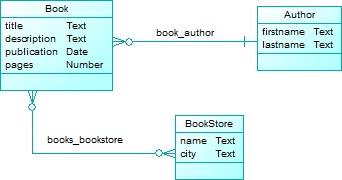
\includegraphics{images/simple_model.png}
	\caption{Modèle simplifié}\label{model-base}
\end{figure}


\subsubsection{Structure du projet}

Le projet se présente sous forme standard Maven :
\begin{itemize}
\item \texttt{src/main/java} : sources JAVA de l'application
\item \texttt{src/main/resources} : ressources et fichiers de configuration
\item \texttt{src/test/java} : sources des tests unitaires
\item \texttt{src/test/resources} : ressources pour les tests unitaires
\end{itemize}

\subsubsection{Maven}

Le fichier maven \texttt{pom.xml} est déjà créé. Il défini une application Java se présentant sous forme de \emph{jar} et ayant comme dépendances, entre autre :
\begin{itemize}
\item Hibernate et le drivers HSQL (version 2.x)
\item Logging (SQL4J via LOG4J)
\item Outils liés à JUNIT (junit, festassert, mockito)
\end{itemize}


\subsubsection{Hibernate}

Hibernate est configuré dans le fichier \texttt{src/main/resources/hibernate.cfg.xml}. Il y est défini :
\begin{itemize}
\item les paramètres de la base de données (url, driver, dialecte SQL)
\item les entités (classes persistantes)
\item le schéma de la base sera supprimé et recréé à chaque exécution du programme\\
\end{itemize}

Ce qui correspond aux paramètres de la \texttt{SessionFactory}. Pour accéder à cette dernière, il faut passer par la classe \texttt{HibernateUtils}.

\subsubsection{SLF4J}
Le loggeur est configuré pour afficher l'ensemble des requêtes SQL exécutées par Hibernate. Le fichier de configuration est \texttt{src/main/resources/log4j.properties}.

\subsubsection{Le modèle}

Les première classes sont déjà écrites pour gagner du temps. Elles sont présentes dans le package \texttt{net.yvesrocher.training.frameworks.dto.model}.\\

Pour rappel, DTO correspond à "Data Transfer Object", ou en français \emph{objet de transfert de données}. Il rassemble différents paramètres de façon logique et objets. Il ne contient \textbf{que} des données (et leurs accesseurs), pas de méthode fonctionnelle !

\subsubsection{Classe \emph{main}}

Afin d'aller droit au but, ce TP se fera directement dans la méthode \texttt{main} (point d'entrée de l'application) et sera lancé via Eclipse.


\subsection{Mon premier mapping de classe}

Dans un premier temps, mappez la classe \texttt{Book} afin qu'elle soit persistante.\\

\begin{enumerate}
\item tester la création d'un nouveau livre
\item modifier le nom de certaines colonnes et de la table, regarder le résultat dans la base de données
\item Insérez plusieurs livres dans la base de données et réaliser quelques recherche dessus : tous,  puis par titre par exemple
\item Charger un livre par son ID et le modifier.\par
Est-ce nécessaire d'appeler la méthode \texttt{saveOrUpdate} après l'avoir modifier ? Est-ce possible de créer un autre objet \texttt{Book}, de lui donner la même ID, et d'appeler la méthode de sauvegarde ?
\end{enumerate}

\subsection{Mapping des classes \texttt{Author} et \texttt{BookStore}}
Dans cette partie, il est conseillée de d'abord travailler sur le mapping d'\texttt{Author} et seulement après passer à \texttt{BookStore}.\\

\begin{enumerate}
\item Mapper les classes \texttt{Author} et \texttt{BookStore}
\item Décommenter les attributs dans la classe \texttt{Book} et mapper les associations
\item Que se passe-t-il quand on sauvegarde un \texttt{Book} qui est lié à un auteur ? Inversement ?
\item Modifier un livre ou un auteur, en le chargeant via son ID, puis en créant une nouvelle instance avec la même ID.
\end{enumerate}

\subsection{Quelques idées de requêtes de recherche}
\begin{itemize}
\item Recherche de livres à partir de l'ID de l'auteur
\item Recherche de livres à partir d'un nom d'auteur
\item Recherche des auteurs dont des ouvrages sont présents dans une ville (on connait les villes des librairies).
\item Recherche des auteurs qui ont écrit au moins 2 livres
\item Recherche des livres présents dans au moins 2 libraires
\item Recherche des auteurs dont au moins 2 livres sont présents dans un librairie données.
\end{itemize}


\section{Pour aller plus loin ...}
Pour aller plus loin, mapper le modèle présenté sur la figure \ref{model-real} \vpageref{model-real}.\\

On intègre l'idée de BookCopy : un exemplaire d'un livre.

\begin{figure}[ht]
	\center
	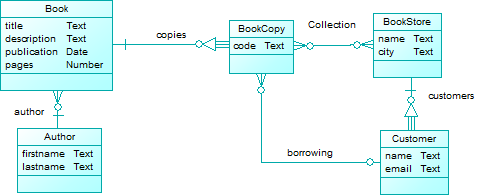
\includegraphics{images/model_real.png}
	\caption{Modèle complet}\label{model-real}
\end{figure}


\section{Pour aller encore plus loin}

Gestion de l'héritage : introduction de la classe \texttt{Person} dont héritent \texttt{Customer} et \texttt{Author}. Voir figure \ref{model-inheritance} \vpageref{model-inheritance}.\\


\begin{figure}[ht]
	\center
	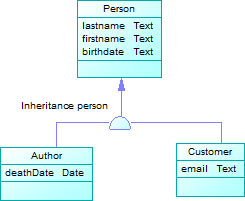
\includegraphics{images/model_inheritance.png}
	\caption{Modèle avec héritage}\label{model-inheritance}
\end{figure}

\begin{enumerate}
\item Tester les différentes stratégie d'héritage (une seule table, 2 tables (une par classe), 3 tables (mutualisation des paramètres communs dans une table).
\item Pour chaque stratégie, essayer quelques requêtes : recherche d'auteurs ou de clients, puis recherche de personne en générale.
\item Un héritage au sens base de données est-il une si bonne idée dans ce cas ? Trouver une solution sans héritage en base à proprement parlé.
\end{enumerate}

\clearpage
\section{Annexes}
\lstset{language=XML}

\subsection{Configuration du poste}

\subsubsection{Configuration de \emph{Maven} : \texttt{.m2/settings.xml}}\label{mvn-settings}
\begin{lstlisting}
<settings>
  <proxies>  
    <proxy>
      <active>true</active>
      <protocol>http</protocol>
      <host>yrproxy01</host>
      <port>8080</port>
      <username>user</username>
      <password>password</password>
    </proxy>
    <proxy>
      <active>true</active>
      <protocol>https</protocol>
      <host>yrproxy01</host>
      <port>8080</port>
      <username>user</username>
      <password>password</password>
    </proxy>    
  </proxies>  
</settings>

\end{lstlisting}


\end{document}